\section{natural alternating diagram}

Suppose we have a positive braid word $\omega$, then we can draw the associated braid diagram($i_1,\cdots,i_{n-1}: [0,1]_{x}\rightarrow [0,1]_{x} \times (0,1)_{z}$ where $i_{k}$ are smooth sections of the projection $[0,1]_{x} \times (0,1)_{z} \rightarrow [0,1]_{x}$) on $[0,1]_{x} \times (0,1)_{z}$ and its cylindrical closure $S^{1}_{x} \times (0,1)_{z}$. For example, if $\omega = s_{1}s_{1}$, a braid word on $3$ strand, then the cylindrical closure of the associated braid diagram is shown in the figure below.

\begin{figure}[H] 
    \centering
    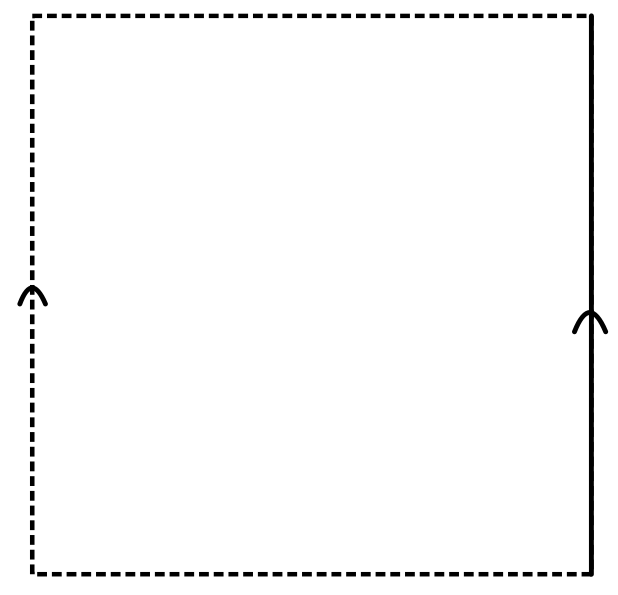
\includegraphics[scale = 0.55]{diagrams/natural_alternating_diagrams/1.png}
    \caption{}
    \label{fig:your-label}
\end{figure}


We will specify co-orientations of $i_1, \cdots, i_{n-1}$ so that we can think of the cylindrical closure of the braid word as the the front projection of a Legendrian knot living inside the co-circle bundle of the cylindrical closure.

Let $x_0 \in [0,1]$, we define the co-orientation at $i_k(x_0)$ to be $\xi = adx + cdz$ so that $\xi$ vanishes at $\frac{di_k}{dt}|_{x=x_0}$, $||(a,c)||= 1$, and $c>0$. This can be visually represented as hairs pointing upward(i.e. $c>0$).

\begin{figure}[H] 
    \centering
    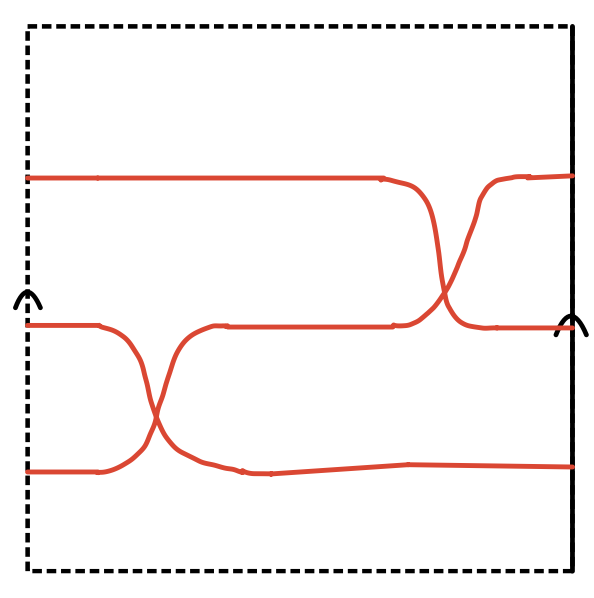
\includegraphics[scale = 0.55]{diagrams/natural_alternating_diagrams/2.png} 
    \caption{}
    \label{fig:your-label}
\end{figure}

Suppose we have a Riemann sphere $M$ with two punctures at $0$ and $\infty$. $M$ is diffeomorphic to the boundaryless cylinder as shown in the figure below.

\begin{figure}[H]
    \centering
    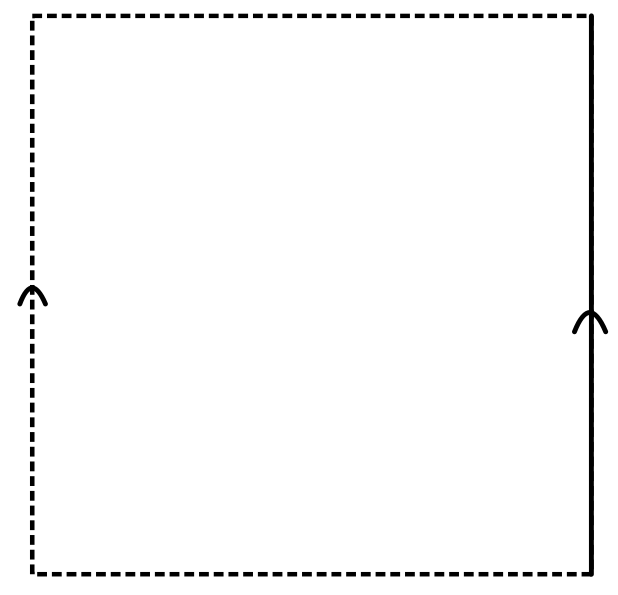
\includegraphics[scale = 0.55]{diagrams/natural_alternating_diagrams/3.png} 
    \caption{}
    \label{fig:your-label}
\end{figure}

There are two distinguished ways of embedding the cylindrical closure of $\omega$ into $M$. We can embed the cylindrical closure onto the hemisphere containing $0$($\infty$ resp.), i.e. the lower hemisphere(upper hemisphere resp.), in such a way that the embedding extends

\begin{enumerate}[label = (\roman*)]
\item to $S^1 \times \{ 0 \}$) as an isomophism onto the equator of $M$
\item to  $S^1 \times \{ 1 \}$ as a constant map to $0$($\infty$ resp.)
\end{enumerate}

\begin{figure}[H]
    \centering
    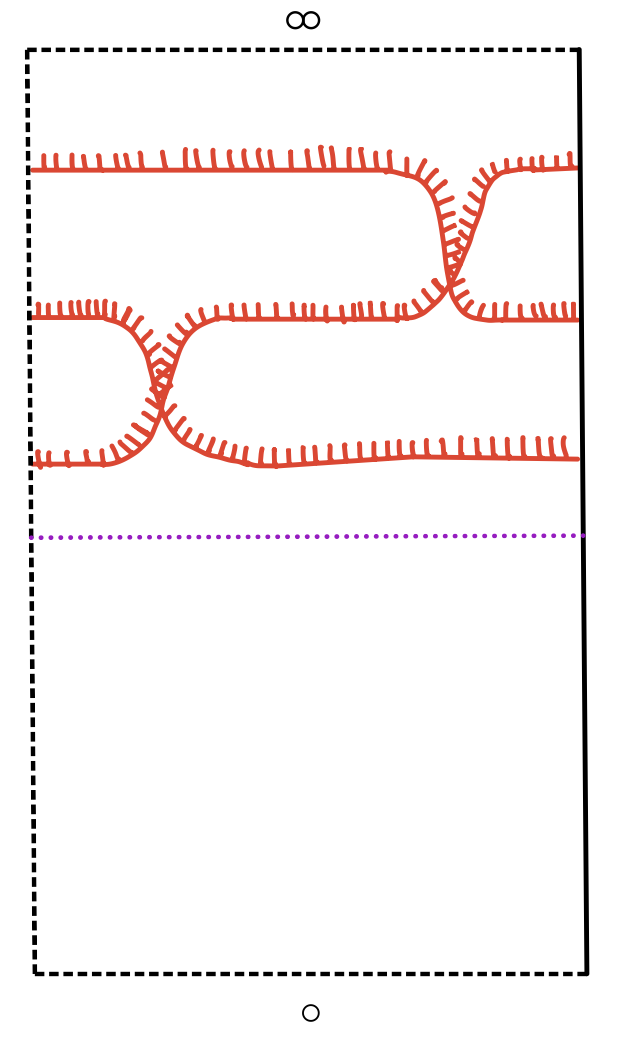
\includegraphics[scale = 0.55]{diagrams/natural_alternating_diagrams/4-1.png} 
    \caption{}
    \label{fig:your-label}
\end{figure}

\begin{figure}[H] 
    \centering
    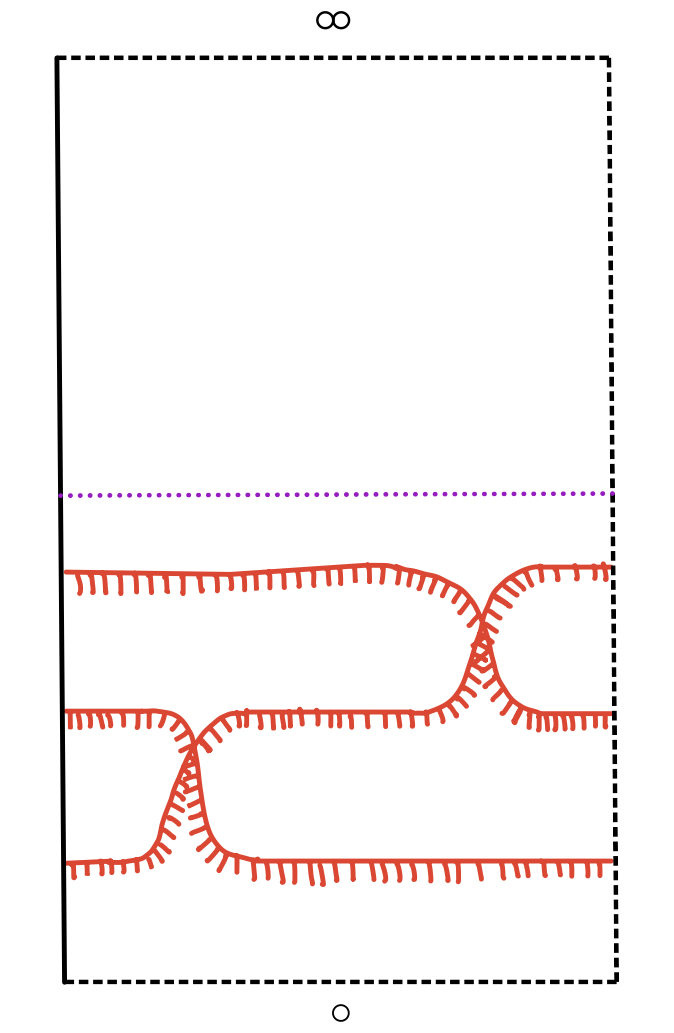
\includegraphics[scale = 0.55]{diagrams/natural_alternating_diagrams/4-2.png} 
    \caption{}
    \label{fig:your-label}
\end{figure}

Suppose we have a positive braid word $\omega$ on $n$ strands, we have the following associated objects: 
\begin{itemize}
\item $M$: A Riemann sphere with two punctures at $0$ and $\infty$

\item $\Phi_0 : \coprod_{i=1}^{n} S^1 \rightarrow  M$: the front projection induced by the embedding of the cylindrical closure of the trivial braid word onto the lower hemisphere

\item $\xi_0$: the co-orientation of $\Phi_0$

\item $\Phi_\infty : \coprod_{i=1}^{m} S^1 \rightarrow M$ (where $m \leq n$): the front projection given by the embedding of the cylindrical closure of the braid word $\omega$ onto the upper hemisphere

\item $\xi_\infty$ : the co-orientation of $\iota_\infty$
\end{itemize}

To simplify the notation, we will denote the pair $(\Phi_0,\xi_0)$($(\Phi_\infty,\xi_\infty)$ resp.) as $\Lambda_0$($\Lambda_\infty$ resp.). Also, we will abuse $\Lambda_0$($\Lambda_\infty$ resp.) to denote the Legendrian associated to the pair $(\Phi_0,\xi_0)$($(\Phi_\infty,\xi_\infty)$ resp.).

Now fix a positive braid word $\omega$ and the object $(M,\Lambda_0,\Lambda_\infty)$ associated with it which we call the separated diagram of $\omega$. I will define a natural alternating braid diagram $(M,\Lambda'_0,\Lambda'_\infty)$ whose associated Legendrian is Legendrian isotopic to the Legendrian associated with $(M,\Lambda_0,\Lambda_\infty)$. I will construct an explicit Legendrian isotopy between them. Furthermore, I will construct cobordisms between constructible sheaves singular supported on $(M,\Lambda_0,\Lambda_\infty)$ and $(M,\Lambda'_0,\Lambda'_\infty)$ which will be the main result of this chapter. The isotopy will be only applied to $\Lambda_0$, so the $\Lambda_\infty$ will remain fixed i.e. $\Lambda_\infty = \Lambda'_\infty$.

First, let's draw $\Lambda'_\infty$ as in red on $M$ as follows :

\begin{figure}[H] 
    \centering
    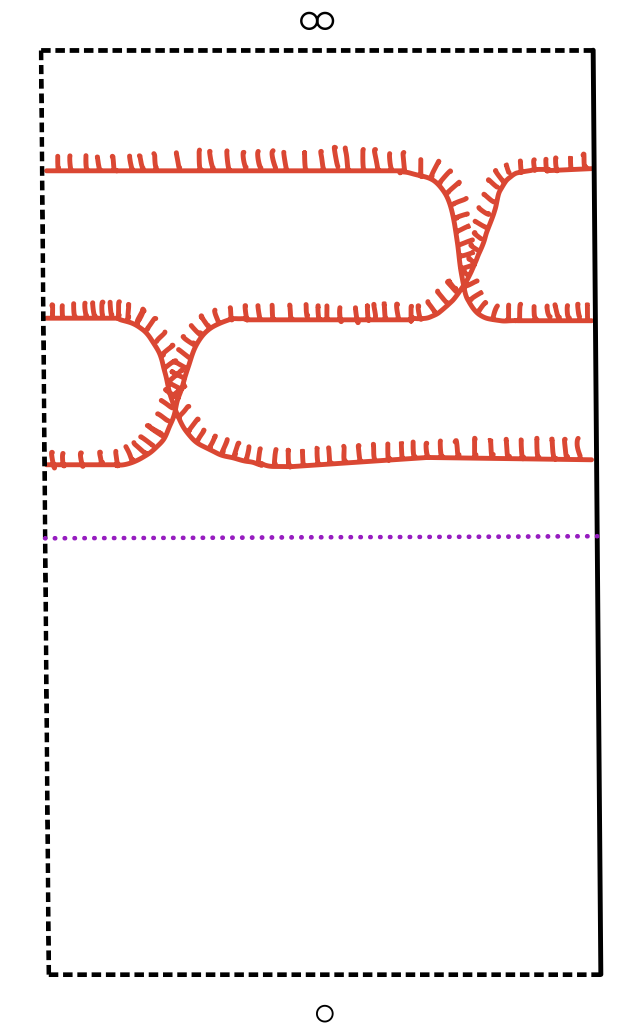
\includegraphics[scale = 0.55]{diagrams/natural_alternating_diagrams/5.png}
    \caption{}
    \label{fig:your-label}
\end{figure}

Now on the above diagram, let's draw $\Lambda'_0$ the part that is Legendrian isotopic to $\Lambda_0$ in blue. But before that, we need some definitions.

\begin{definition}
Suppose $\omega = s_{1_1},..., s_{i_k}$, then the cylindrical closure can be parsed into a concatenation of k mutually disjoint regions where $i^{th}$ region containing a part of the braid diagram corresponding to the generator $s_{i_j}$ shown in the figure below. We call the region corresponding to $s_{i_j}$ as the $j^{th}$ generator region(also its image under the embedding into $M$).
\end{definition}

Below is the picture of the $1^{st}$ generator region of the cylindrical closure of $\omega = s_1 s_2$.

\begin{figure}[H] 
    \centering
    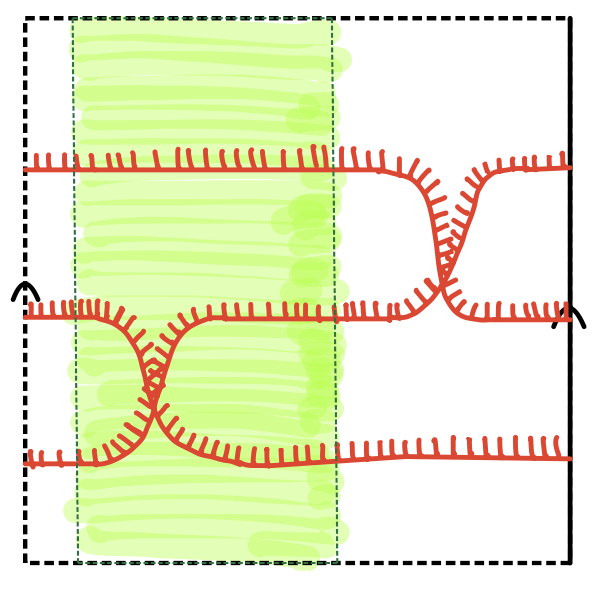
\includegraphics[scale = 0.55]{diagrams/natural_alternating_diagrams/6-1.png}
    \caption{}
    \label{fig:your-label}
\end{figure}

Below is the picture of the $2^{nd}$ generator region of the cylindrical closure of $\omega = s_1 s_2$.

\begin{figure}[H] 
    \centering
    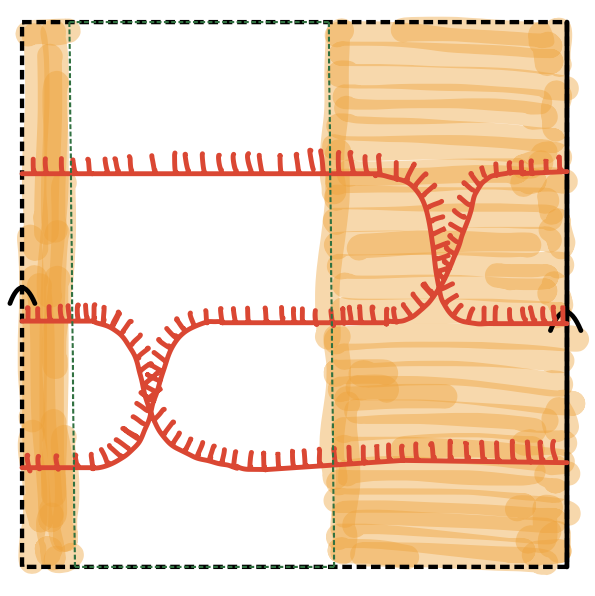
\includegraphics[scale = 0.55]{diagrams/natural_alternating_diagrams/6-2.png}
    \caption{}
    \label{fig:your-label}
\end{figure}

\begin{definition}
Suppose we set-theoretically subtract the union of all generator regions from the cylinder, we get $k$ connected components. That is, for each $j = 1,...,k$, we have one component in between $j^{th}$ and ($j+1$ (mod $k$))$^{th}$ regions. We call the neighborhood of this component inside the cylinder as  $j^{th}$ inter-generator region(also its image inside the cylinder under the embedding into $M$).

\begin{itemize}
\item inter-generator regions do not contain any crossing
\item inter-generator regions are mutually disjoint
\item $j^{th}$ intergenerator region intersects with $j^{th}$ and $j+1^{th}$(modulo $k$) generator region
\end{itemize}
\end{definition}

Below is the picture of the $1^{st}$ inter-generator region of the cylindrical closure of $\omega = s_1 s_2$.

\begin{figure}[H] 
    \centering
    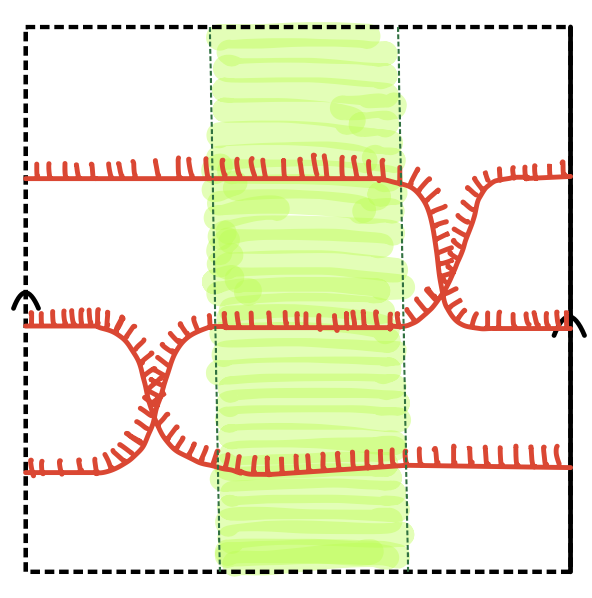
\includegraphics[scale = 0.55]{diagrams/natural_alternating_diagrams/7-1.png}
    \caption{}
    \label{fig:your-label}
\end{figure}

Below is the picture of the $2^{nd}$ generator region of the cylindrical closure of $\omega = s_1 s_2$.

\begin{figure}[H]
    \centering
    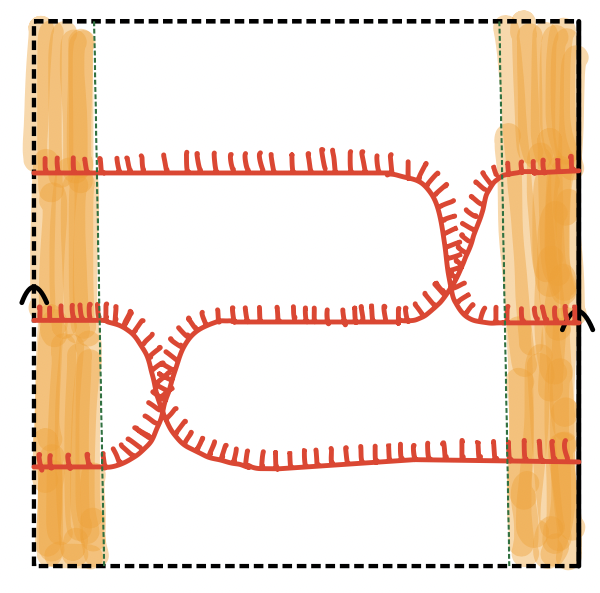
\includegraphics[scale = 0.55]{diagrams/natural_alternating_diagrams/7-2.png}
    \caption{}
    \label{fig:your-label}
\end{figure}

Now I will draw $\Lambda'_0$ for each generator region so that they glue up to the whole $\Lambda'_0$. 

First, we restrict the diagram to $j^{th}$ generator region, we have the following diagram: Note that $i_j^{th}$ and $i_{j}+1^{th}$ strands cross each other and all the other strands are horizontal.

\begin{figure}[H] 
    \centering
    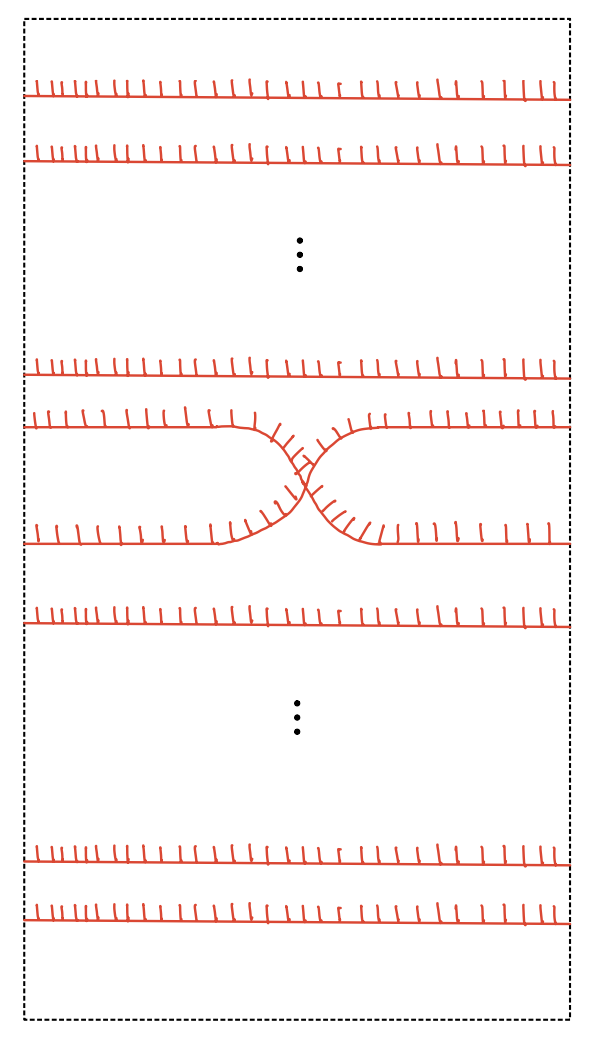
\includegraphics[scale = 0.55]{diagrams/natural_alternating_diagrams/8.png} 
    \caption{}
    \label{fig:your-label}
\end{figure}


We label the strands from bottom to top using integers from $1$ to $n$ with reference to the left end points. This is the strand labelling scheme that I will use throughout this chapter.


I will draw $\Lambda'_0$ as blue strand on it as follows :

\begin{itemize}
\item $l^{th}$ blue strand starts from the midpoint of the starting points of $l-1^{th}$ and $l^{th}$ red strands and ends at the midpoint of the end points of $l-1^{th}$ and $l^{th}$ red strands

\item if $l \neq i_j$ and $i\neq i_j +1$, then along the way the $l^{th}$ blue strand crosses up and down once

\item if $l = i_j +1$, $l^{th}$ blue strand crosses $l^{th}$ red strand up in the part before the crossing and then crosses $l-1^{th}$ red strand down in the part after the crossing.

\item if $l = i_j$, $l^{th}$ blue strand crosses $l^{th}$ red strand up and down in the part before the crossing and then crosses $l+1^{th}$ red strand up and down in the part after the crossing.
\end{itemize}

The picture below overlays $\Lambda'_0$, drawn in blue strands with hairs pointing downward, on the previous diagram.

\begin{figure}[H] 
    \centering
    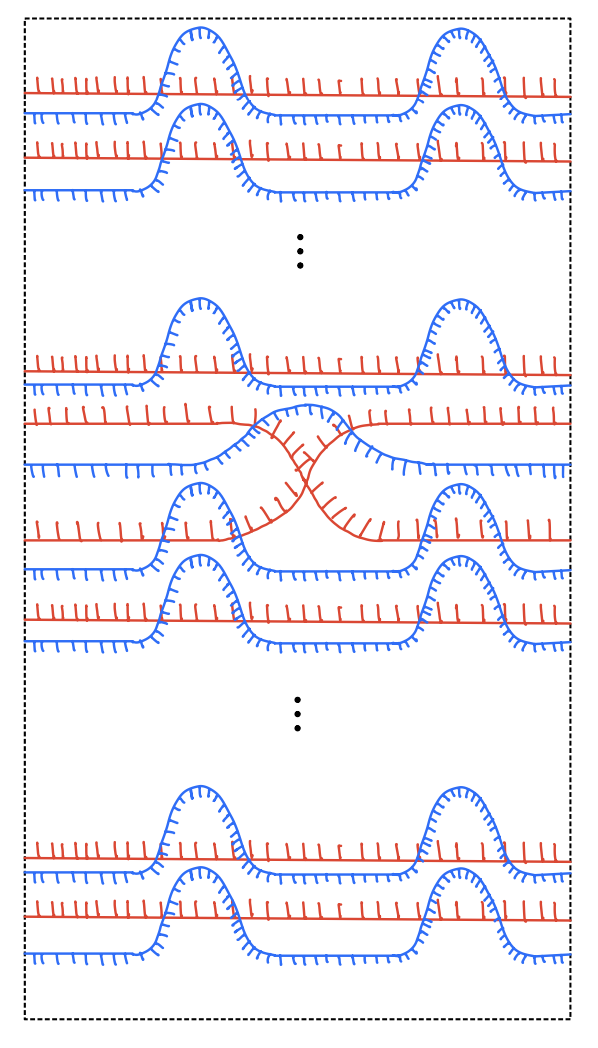
\includegraphics[scale = 0.55]{diagrams/natural_alternating_diagrams/9.png}
    \caption{}
    \label{fig:your-label}
\end{figure}

For the full alternating strand diagram, we take the closure of blue strands from the generator regions so that the end points from the bordering regions coincide.

The picture below shows how the global natural alternating strand diagram associated with $\omega = s_1 s_2$ looks like after gluing together local alternating strand diagrams of $s_1$ and $s_2$.

\begin{figure}[H] 
    \centering
    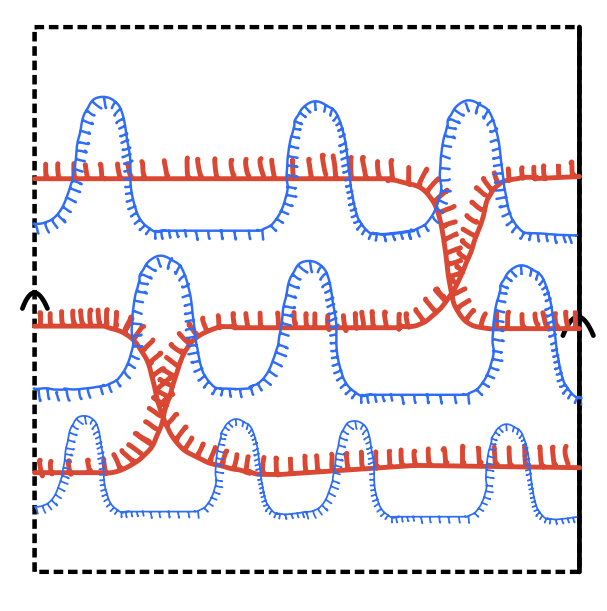
\includegraphics[scale = 0.55]{diagrams/natural_alternating_diagrams/10.png} 
    \caption{}
    \label{fig:your-label}
\end{figure}

\begin{theorem}
The above defined strand diagram is alternating
\end{theorem}

\begin{proof}
we will denote
 
\begin{itemize}
\item the region with all the hairs pointing outward as $\circ$
\item the region with all the hairs pointing inward as $\bigtriangleup$
\item else with $\times$
\end{itemize}

for the generator region we have the following figure :

\begin{figure}[H] 
    \centering
    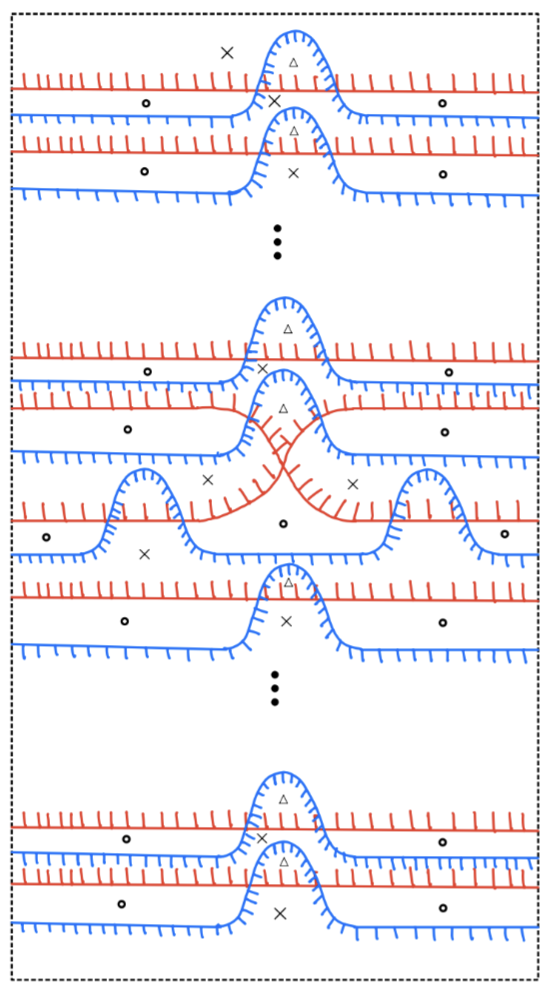
\includegraphics[scale = 0.55]{diagrams/natural_alternating_diagrams/11.png}
    \caption{}
    \label{fig:your-label}
\end{figure}

The above marking extends to the inter-generator region, we have the following figure:

\begin{figure}[H] 
    \centering
    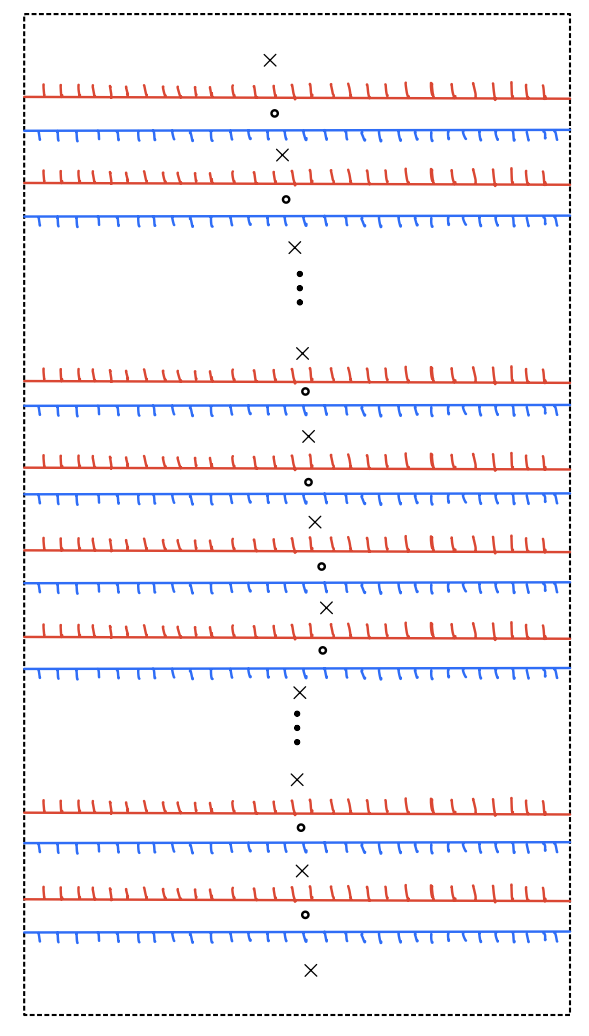
\includegraphics[scale = 0.55]{diagrams/natural_alternating_diagrams/12.png}
    \caption{}
    \label{fig:your-label}
\end{figure}

for each crossing, it satisfy the alternating condition. This diagram is indeed alternating.
\end{proof}
\pagebreak